\documentclass[
portrait,
a0paper,
%margin=5mm,
%draft
]
{baposter}
%
% load packages
% already loaded some useful packages for figures, tables and layout
% not all are needed to run this minimal example
\usepackage{graphicx}
\usepackage[percent]{overpic}
\usepackage[detect-weight]{siunitx}
\usepackage{tabto}
\usepackage{booktabs}
\usepackage{amsmath}
\usepackage{float}
\usepackage{multirow}
\usepackage{url}
\usepackage{enumitem}
\usepackage{qrcode}
% add additional packages you need here
\usepackage{tikz}
\usetikzlibrary{positioning}
\usepackage{listings}
\lstset{basicstyle=\ttfamily\tiny, breaklines=true, frame=single, backgroundcolor=\color{TUMlightgray!40}}
%
% for now usig bibitem, but if you want ...
%\usepackage[backend=biber]{biblatex} 
%
% customizing 
\newlength{\mytextsize}
\newcommand\e{\cdot 10^}
\setlength{\unitlength}{1.0cm}
%
%%%%%%%%%%% TUM COLORS %%%%%%%%%%%%%%%%
%%% main colors %%%
\definecolor{TUMblue}{RGB}{0, 101, 189}
%%% Secondary colors %%%
\definecolor{TUMdarkblue}{rgb}{0.00, 0.32, 0.576}
\definecolor{TUMlightblue}{rgb}{0.392, 0.627, 0.784}
\definecolor{TUMlighterblue}{rgb}{0.596, 0.776, 0.917}
\definecolor{TUMgray}{rgb}{0.6, 0.6, 0.6}
\definecolor{TUMlightgray}{rgb}{0.855, 0.843, 0.796}
%%% Emphasis %%%
\definecolor{TUMorange}{rgb}{0.89, 0.447, 0.133}
\definecolor{TUMgreen}{rgb}{0.635, 0.678, 0.00}

% fonts
\usepackage[scaled]{helvet}
\renewcommand*\familydefault{\sfdefault}
%
%
%##################################################################################
\begin{document}
%##################################################################################
\begin{poster}
{
  % options
  grid=false,%true,
  background=plain,
  bgColorOne=white,
  columns=6, % for flexibility changing 2/3 columns with columnspan
  eyecatcher=false,
  borderColor=TUMdarkblue,
  headerColorOne=TUMdarkblue, %white,
  headershade=plain,
  %headerColorTwo=white,
  headerborder=open,
  % for rectangular boxes change the next two options, rectangular header will cause left aligning of box title 
  textborder=rounded, %rectangle,
  headershape=rounded, %rectangle,
  headerfont=\bf\Large,
  boxshade=none,
  headerFontColor=white
}
{
  %eyecatcher ...
}
{
  %poster title
  % first put graphics for header
  \hspace*{-0.5mm}
  \begin{picture}(23.7, 3)
  \fboxsep0pt
  \put(-0.196, -0.6){\colorbox{TUMdarkblue}{\rule[96pt]{675.82pt}{0pt}}}
  \thicklines
  % minipage box for title and authors
  \put(2.55, 2.35){
    \begin{minipage}[t][96pt]{0.75\textwidth}
    % centering
    \begin{center}
    % Title
    % use \LARGE instead of \Huge for long titles, you might need to modify distances or number of lines
    % for one line title
    %\ \vspace{0.15cm}\\
    %\huge\bf\color{white}\selectfont Single Line Title \vspace{0.4cm}\\ 
    % for two line title
    \huge\bf\color{white}\selectfont Bayesian Neural Networks \\ 
    \huge\bf\selectfont Implementations Using Python Libraries \vspace{0.15cm} \\ 
    \small Masterpraktikum - Formal Methods for AI-Enabled Cyber-Physical Systems \\
    \small Supervisor: Laura L\"utzow and Victor Schulte
    %\small C.\ Author, Institute \\
    %\small D.\ Author, Institute
    % two lines
    \end{center}
  \end{minipage}}
  %  
  % left:
  %\put(0.32,-0.24){\includegraphics[height=75pt]{logos/LogoOutline-White.eps}}
  % right:
  %\put(18.18,1.25){\color{white}\qrcode[hyperlink,height=50pt]{https://www.ce.cit.tum.de/cps/home/}}
  \put(18.8,-0.2){\large\bf\color{white}Unique Group Identifier}
  \put(20.4,0.9){
\includegraphics[height=40pt]{logos/TUM_Logo_weiss.png}}
  %% DO NOT FORGET to replace QR code link and Poster ID !
  % % poster id + qr code, for example at IPAC
  % Modify links!!!
  % left
  %\put(0.2,0.75){
\includegraphics[height=50pt]{logos/face.png}}
  %\put(-0.2,0.45){\begin{minipage}[t][]{70pt}
  %  \begin{center}
  %  \large\bf\color{white}\selectfont Gabriel \\
  %  \large\bf\selectfont Carpio Saez de Nanclares \\
  %  \end{center}
  %\end{minipage}}

  \put(2.0,0.75){
\includegraphics[height=50pt]{logos/face.png}}
  \put(-1.5,0.45){\begin{minipage}[t][]{250pt}
    \begin{center}
    \large\bf\color{white}\selectfont Gabriel \\
    \large\bf\selectfont Carpio Saez de Nanclares \\
    \end{center}
  \end{minipage}}

  %\put(5,0.75){
\includegraphics[height=50pt]{logos/face.png}}
  %\put(4.7,0.45){\begin{minipage}[t][]{70pt}
   % \begin{center}
    %\large\bf\color{white}\selectfont FirstName \\ 
    %\large\bf\selectfont LastName \\ 
    %\end{center}
  %\end{minipage}}
  % right
  %\put(21.02,-0.25){\large\bf\color{white}Poster ID}
  %\put(21,1.1){\color{white}\qrcode[hyperlink,height=.08\textwidth]{https://gitlab.cern.ch/mkoopman/templates}}
  \end{picture} 
}
{
	%poster authors, already in title
}
{
	%logo, already in title
}
%
% three part footnote box with references, logos, contact infos
%
\headerbox{}{headershape=rectangle, name=foottext, column=0, span=6, above=bottom, textborder=none, borderColor=TUMdarkblue,  boxheaderheight=1pt}{
  \vspace{.2cm}
  $\quad$\textbf{\small\color{TUMdarkblue}KEY REFERENCES}\\[2pt]
  \renewcommand{\section}[2]{}
  \begin{minipage}[t]{0.48\linewidth}\begin{tiny}
    \begin{thebibliography}{9}
    \setlength{\itemsep}{0pt}\setlength{\parsep}{0pt}\setlength{\topsep}{0pt}
      \bibitem[1]{goan2020bayesian}
      E.~Goan, C.~Fookes, ``Bayesian Neural Networks: An Introduction and Survey,'' \emph{Case Studies in Applied Bayesian Data Science}, Springer, 2020.
      \bibitem[2]{murphy2023pml}
      K.~P.~Murphy, \emph{Probabilistic Machine Learning: Advanced Topics}, MIT Press, 2023.
    \end{thebibliography}
  \end{tiny}\end{minipage}\hfill
  \begin{minipage}[t]{0.48\linewidth}\begin{tiny}
    \begin{thebibliography}{9}
    \setlength{\itemsep}{0pt}\setlength{\parsep}{0pt}\setlength{\topsep}{0pt}
      \bibitem[3]{intel2021bayesiantorch}
      Intel Labs, \texttt{bayesian-torch}: A Library for Bayesian Neural Network Layers, 2021.
      \bibitem[4]{daxberger2021laplace}
      E.~Daxberger et al., ``Laplace Redux: Effortless Bayesian Deep Learning,'' \emph{NeurIPS}, 2021.
    \end{thebibliography}
  \end{tiny}\end{minipage}
}
%
% and now the standard boxes on the poster
% choose between 2 or 3 column layout here!
% for 2 column layout use column=0 and column=3, respectively (always span=3)
% for 3 column layout use column=0, column=2 and column=4, respectively (always span=2)
% or go with 6 columns and column span ... 
%
% in the following is here a simple example for two column layout with
% three boxes on the left: motivation, left box 1, left box 2 and
% two boxes on the right: large right box, summary
%
\headerbox{Motivation}{name=motivation, column=0, row=0, span=3}{
  \begin{itemize}[noitemsep,topsep=0pt,parsep=0pt,partopsep=0pt, leftmargin=10pt]
   \item \textbf{Neural Networks (NNs)} are widely used in many applications, but they are often overconfident in their predictions and do not provide uncertainty estimates.
   \item NNs typically get trained in a \textbf{frequentist} manner, which means that the model parameters are fixed point estimates after training. 
   \item \textbf{Bayesian Neural Networks (BNNs)} provide a probabilistic framework for neural networks, allowing for \textbf{uncertainty estimation} in predictions~\cite{goan2020bayesian,murphy2023pml}.
   \item BNNs treat the model parameters as random variables.
\vspace{-0.4cm}
\begin{center}
\resizebox{\linewidth}{!}{%
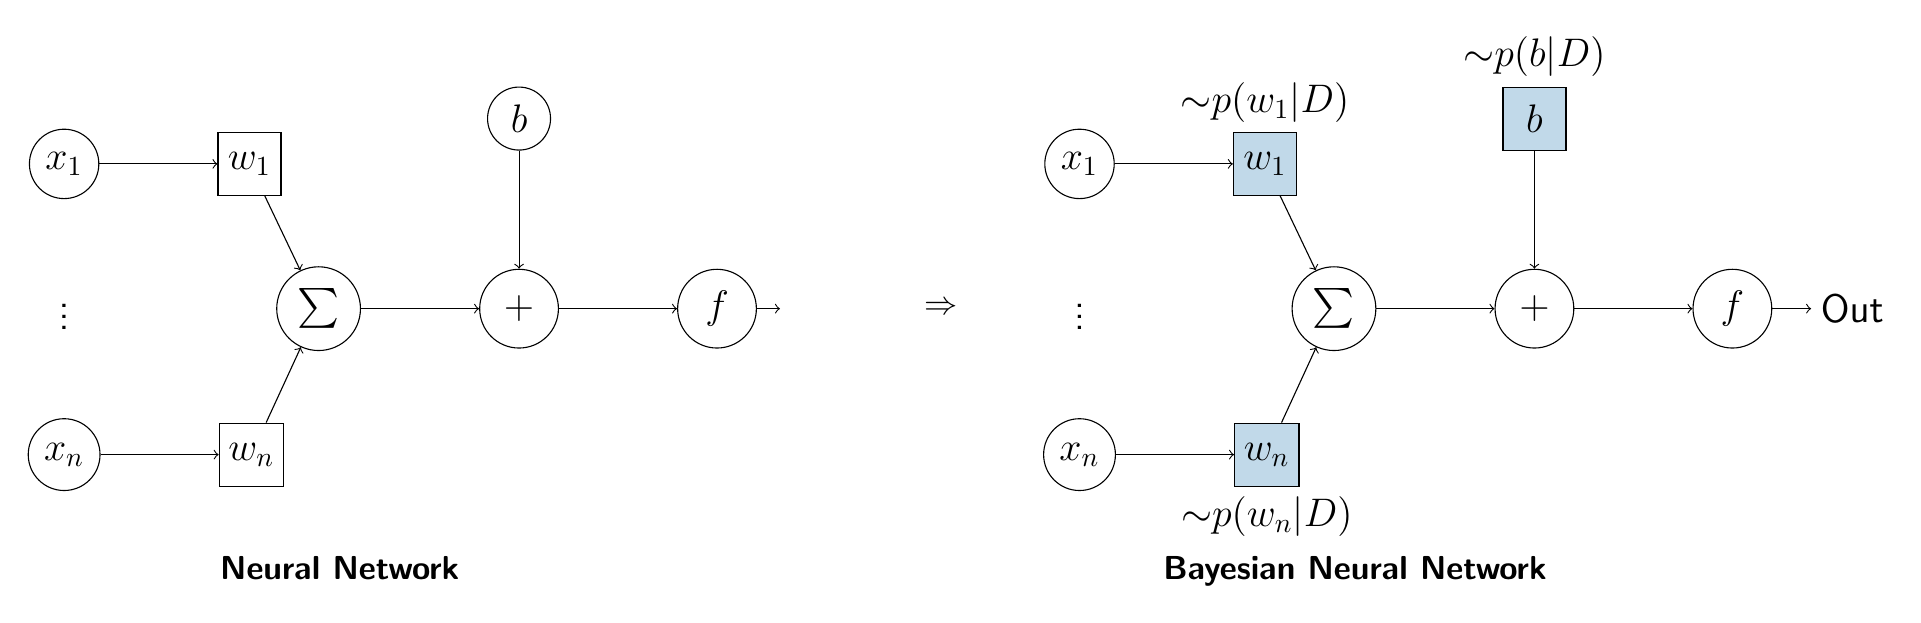
\begin{tikzpicture}[
    font=\Large,
    node distance=1.5cm,
    input/.style={circle, draw, minimum size=0.8cm},
    weight/.style={rectangle, draw, minimum size=0.8cm},
    bweight/.style={rectangle, draw, minimum size=0.8cm, fill=TUMlightblue!40},
    op/.style={circle, draw, minimum size=1cm}
]
% --- Deterministic network (left) ---
\node[input] (X1) {$x_1$};
\node[below=1.0cm of X1] (dots) {$\vdots$};
\node[input, below=1.0cm of dots] (Xn) {$x_n$};
\node[weight, right=1.5cm of X1] (W1) {$w_1$};
\node[weight, right=1.5cm of Xn] (Wn) {$w_n$};
\node[op, right=2.5cm of dots] (Sum) {$\sum$};
\node[op, right=1.5cm of Sum] (Plus) {$+$};
\node[input, above=1.5cm of Plus] (B) {$b$};
\node[op, right=1.5cm of Plus] (Act) {$f$};
\draw[->] (X1) -- (W1);
\draw[->] (Xn) -- (Wn);
\draw[->] (W1) -- (Sum);
\draw[->] (Wn) -- (Sum);
\draw[->] (Sum) -- (Plus);
\draw[->] (B) -- (Plus);
\draw[->] (Plus) -- (Act);
\draw[->] (Act) -- ++(0.8,0);

% --- Arrow between networks ---
\node[right=2.0cm of Act, font=\large] {$\Rightarrow$};

% --- Bayesian network (right) ---
\node[input, right=12cm of X1] (BX1) {$x_1$};
\node[below=1.0cm of BX1] (Bdots) {$\vdots$};
\node[input, below=1.0cm of Bdots] (BXn) {$x_n$};
\node[bweight, right=1.5cm of BX1, label=above:{${\sim}p(w_1|D)$}] (BW1) {$w_1$};
\node[bweight, right=1.5cm of BXn, label=below:{${\sim}p(w_n|D)$}] (BWn) {$w_n$};
\node[op, right=2.5cm of Bdots] (BSum) {$\sum$};
\node[op, right=1.5cm of BSum] (BPlus) {$+$};
\node[bweight, above=1.5cm of BPlus, label=above:{${\sim}p(b|D)$}] (BB) {$b$};
\node[op, right=1.5cm of BPlus] (BAct) {$f$};
\draw[->] (BX1) -- (BW1);
\draw[->] (BXn) -- (BWn);
\draw[->] (BW1) -- (BSum);
\draw[->] (BWn) -- (BSum);
\draw[->] (BSum) -- (BPlus);
\draw[->] (BB) -- (BPlus);
\draw[->] (BPlus) -- (BAct);
\draw[->] (BAct) -- ++(1,0) node[right] {Out};
% Captions
\node[below=0.7cm of Xn,  xshift=3.5cm,  font=\large\bfseries] {Neural Network};
\node[below=0.7cm of BXn, xshift=3.5cm, font=\large\bfseries] {Bayesian Neural Network};
\end{tikzpicture}}
\end{center}
  \end{itemize}  
}
%
%
\headerbox{Approximating the Posterior}{name=vmeas, span=3, below=motivation, column=0}{
  \begin{itemize}[noitemsep,topsep=0pt,parsep=0pt,partopsep=0pt, leftmargin=10pt]
    \item \textbf{Variational Inference (VI)}~\cite{goan2020bayesian,murphy2023pml}: Inference as optimization. Minimizes $\mathrm{KL}[q(\theta)\,\|\,p(\theta|D)]$ by maximizing the \textbf{Evidence Lower Bound (ELBO)}:
      \[\mathcal{L}_\text{ELBO} = \mathbb{E}_{q(\theta)}[\log p(D|\theta)] - \mathrm{KL}[q(\theta)\,\|\,p(\theta)]\]
    \begin{itemize}[noitemsep,topsep=0pt,parsep=0pt,partopsep=0pt, leftmargin=12pt]
      \item \textbf{Bayes by Backprop (BBB)}: Uses the reparameterization trick to allow gradients to flow through stochastic weights. Instead of sampling $w \sim \mathcal{N}(\mu, \sigma^2)$ directly, write
      \[w = \mu + \sigma \odot \hat{\varepsilon}, \quad \hat{\varepsilon} \sim \mathcal{N}(0, I)\]
      making the ELBO differentiable w.r.t.\ the variational parameters $\mu, \sigma$.
      \item \textbf{Flipout}: Reduces gradient variance by applying independent sign-flip matrices $\mathbf{r}_n, \mathbf{s}_n \!\in\! \{-1,+1\}^*$ to the shared perturbation $\Delta\hat{\mathbf{W}}$ per sample:
      \[\hat{\mathbf{W}}_n = \mathbf{W}_{\mathrm{MAP}} + \mathbf{s}_n \odot \Delta\hat{\mathbf{W}} \odot \mathbf{r}_n^\top, \quad \Delta\hat{\mathbf{W}} = \boldsymbol{\sigma} \odot \hat{\boldsymbol{\varepsilon}},\ \hat{\boldsymbol{\varepsilon}} \sim \mathcal{N}(0,\mathbf{I})\]
    \end{itemize}
    \item \textbf{Laplace Approximation}~\cite{goan2020bayesian,murphy2023pml}: Fits a Gaussian to the posterior \emph{post-hoc} using the Maximum A Posteriori (MAP) estimate $\theta_{\mathrm{MAP}}$:
    \begin{itemize}[noitemsep,topsep=0pt,parsep=0pt,partopsep=0pt, leftmargin=12pt]
      \item \textbf{Hessian Computation}: at $\theta_{\mathrm{MAP}}$, compute $H = -\nabla^2 \log p(\theta|D)$, capturing local curvature of the loss landscape.
      \item \textbf{Gaussian Fitting}: Approximate $q(\theta) = \mathcal{N}(\theta;\,\theta_{\mathrm{MAP}},\,H^{-1})$.
    \end{itemize}
  \end{itemize}
}
%
%
\headerbox{The Python Libraries}{name=2ddiag, span=3, below=vmeas, above=foottext, column=0}{
  \begin{itemize}[noitemsep,topsep=0pt,parsep=0pt,partopsep=0pt, leftmargin=10pt]
    \item \textbf{\texttt{bayesian-torch}}~\cite{intel2021bayesiantorch}: Converts to Bayesian via \texttt{dnn\_to\_bnn}.
    \begin{itemize}[noitemsep,topsep=0pt,parsep=0pt,partopsep=0pt, leftmargin=12pt]
      \item \textbf{Method}: Flipout or Bayes by Backprop (BBB).
      \item \textbf{Init}: From scratch, or \textbf{MOPED} (Model Priors Extracted from a pretrained Deterministic DNN).
      \item \textbf{Loss}: ELBO  or AvUC:
      \begin{center}
        $\mathcal{L}_{AvUC} = \tfrac{n_{AU}}{n_{AU}+n_{AC}} + \tfrac{n_{IC}}{n_{IC}+n_{IU}}$
      \end{center}
      \item \textbf{Usage}: \parbox[t]{\linewidth}{\ttfamily\small
        dnn\_to\_bnn(net, \{\\
        \quad "prior\_mu": 0.0, "prior\_sigma": 1.0,\\
        \quad "posterior\_mu\_init": 0.0, "posterior\_rho\_init": -3.0,\\
        \quad "type": model\_type, \quad\textit{\# flipout or reparameterization}\\
        \quad "moped\_enable": moped, "moped\_delta": moped\_delta,\})
      }
    \end{itemize}
    \item \textbf{\texttt{laplace-torch}}~\cite{daxberger2021laplace}: Post-hoc wrapper around any trained model.
    \begin{itemize}[noitemsep,topsep=0pt,parsep=0pt,partopsep=0pt, leftmargin=12pt]
      \item \textbf{Scope}: Last layer, subset of weights, or all weights.
      \item \textbf{Hessian}: Full, diagonal, or Kronecker-factored (\texttt{kron}).
      \item \textbf{Prior tuning}: Optimize prior precision via marginal likelihood or grid search.
      \item \textbf{Usage}: \parbox[t]{\linewidth}{\ttfamily\small
        la = Laplace(model, "regression",\\
        \quad subset\_of\_weights="last\_layer",\\
        \quad hessian\_structure="kron")\\
        la.fit(train\_loader)\\
        la.optimize\_prior\_precision(method="marglik")\\
        pred\_mean, pred\_var = la(x\_test)
      }
    \end{itemize}
  \end{itemize}
}
%
%
\headerbox{Experiments}{name=resolution, span=3, row=0, column=3}{
  Three datasets:
  \begin{itemize}[noitemsep,topsep=0pt,parsep=0pt,partopsep=0pt, leftmargin=10pt]
    \item \textbf{Two moons:} a 2D \textit{classification} toy dataset.
    \item \textbf{Sinusoidal function:} a 1D \textit{regression} toy dataset.
    \item \textbf{PovertyMap:} a \textit{regression} satellite imagery dataset for wealth index prediction.
  \end{itemize}
  \vspace{2pt}
  \begin{center}
  \begin{minipage}[t]{0.26\linewidth}\centering
    \includegraphics[height=4cm,width=\linewidth,keepaspectratio]{figures/two_moons_dataset.png}\\[-2pt]
    {\tiny Two Moons}
  \end{minipage}\hfill
  \begin{minipage}[t]{0.26\linewidth}\centering
    
\includegraphics[height=4cm,width=\linewidth,keepaspectratio]{figures/povertymap_samples.png}\\[-2pt]
    {\tiny PovertyMap}
  \end{minipage}\hfill
  \begin{minipage}[t]{0.44\linewidth}\centering
    
\includegraphics[height=4cm,width=\linewidth,keepaspectratio]{figures/sinusoid_dataset.png}\\[-2pt]
    {\tiny Sinusoid}
  \end{minipage}
  \end{center}
  \vspace{2pt}
  \noindent\textbf{Two Moons results:}\\[1pt]
  \noindent\begin{minipage}[t]{0.48\linewidth}\centering
    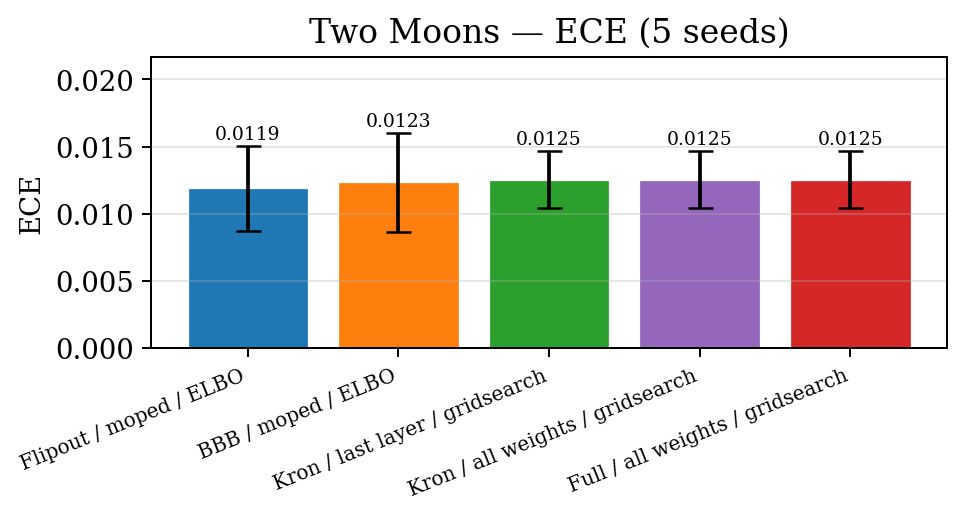
\includegraphics[height=3.4cm,width=\linewidth,keepaspectratio]{figures/merged_tm_ece.png}\end{minipage}\hfill
  \begin{minipage}[t]{0.48\linewidth}\centering
    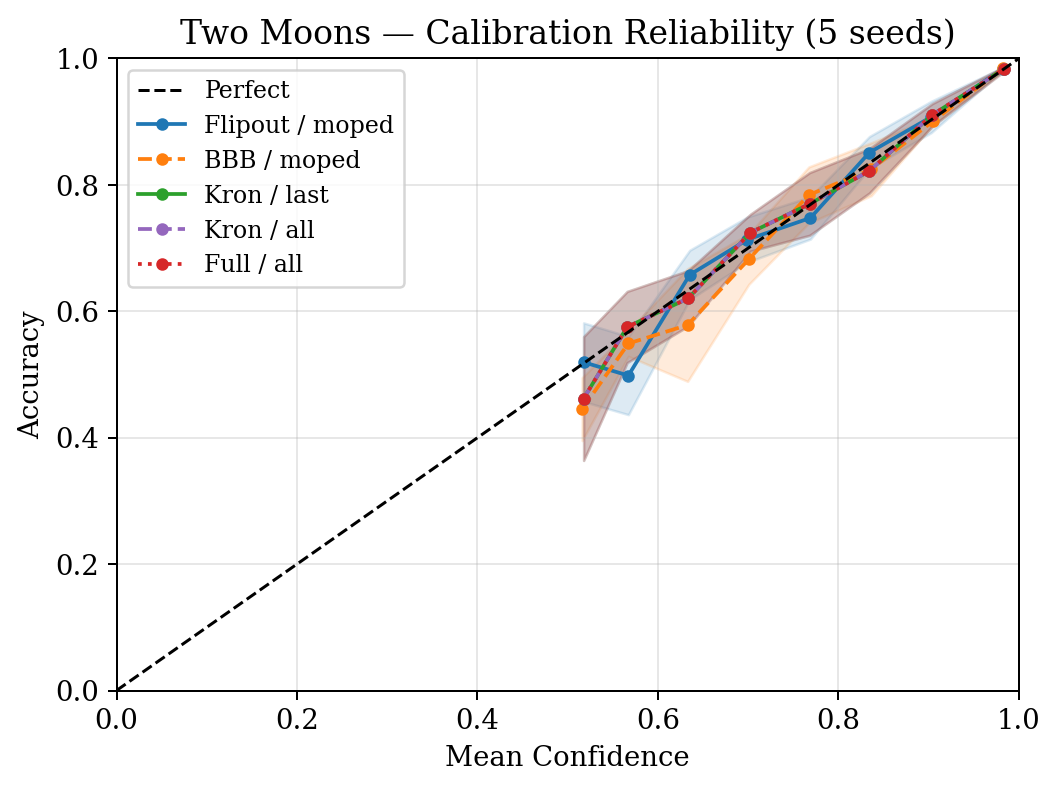
\includegraphics[height=3.4cm,width=\linewidth,keepaspectratio]{figures/reliability_tm_all_variants.png}\end{minipage}
  \vspace{2pt}
  \noindent\textbf{PovertyMap results:}\\[1pt]
  \noindent\begin{minipage}[t]{0.48\linewidth}\centering
    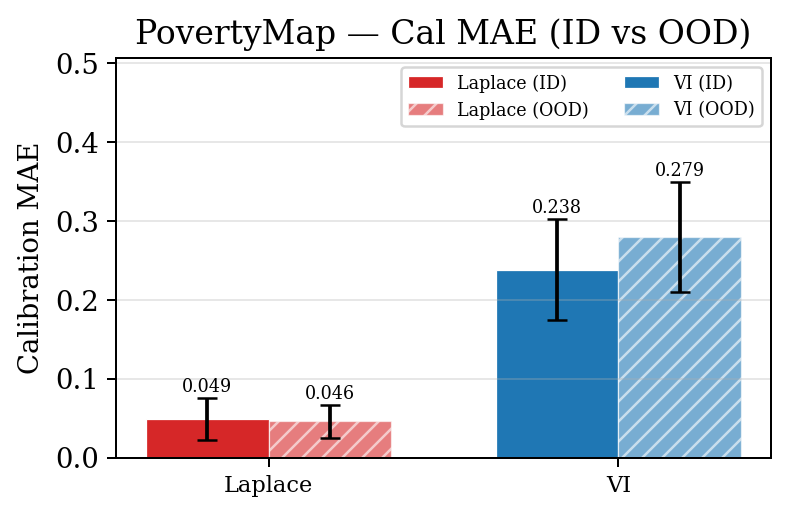
\includegraphics[height=3.4cm,width=\linewidth,keepaspectratio]{figures/cmp_lbnn_pov_cal_mae.png}\end{minipage}\hfill
  \begin{minipage}[t]{0.48\linewidth}\centering
    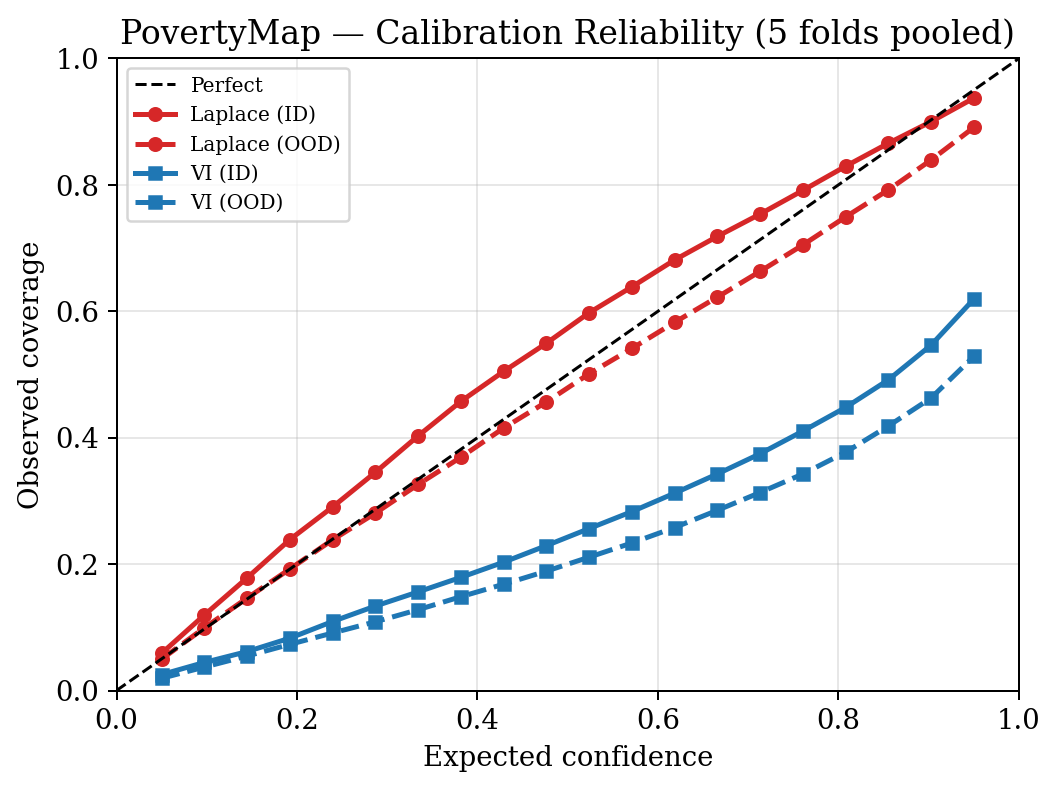
\includegraphics[height=3.4cm,width=\linewidth,keepaspectratio]{figures/reliability_povertymap.png}\end{minipage}
  \vspace{2pt}
  \noindent\textbf{Sinusoidal results:}\\[1pt]
  \noindent\begin{minipage}[t]{0.48\linewidth}\centering
    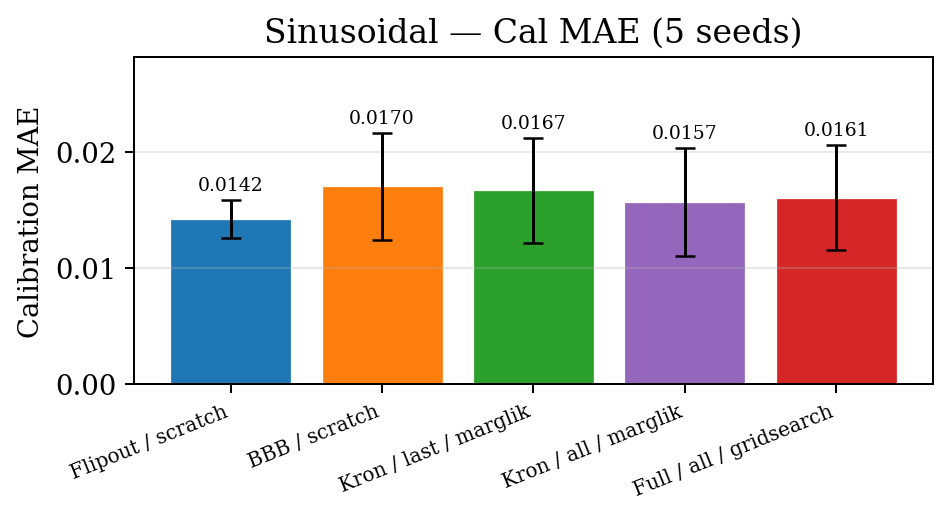
\includegraphics[height=3.4cm,width=\linewidth,keepaspectratio]{figures/merged_sin_cal_mae.png}\end{minipage}\hfill
  \begin{minipage}[t]{0.48\linewidth}\centering
    
\includegraphics[height=3.4cm,width=\linewidth,keepaspectratio]{figures/reliability_sin_all_variants.png}\end{minipage}
  \vspace{4pt}
  \noindent\textbf{Training \& Inference Time:}
  \vspace{2pt}

  \noindent\resizebox{\linewidth}{!}{%
  \begin{tabular}{llrrrr}
    \toprule
    \textbf{Dataset} & \textbf{Method} & \textbf{Fit/Train (s)} & \textbf{LA Tune (s)} & \textbf{Inference (s)} & \textbf{ECE} \\
    \midrule
    \multirow{6}{*}{\shortstack[l]{Two Moons\\{\small MAP: $67.4\!\pm\!31.3$\,s}}}
                                & Flipout / scratch / ELBO  & $32.8 \pm 11.0$          & ---                    & $0.047 \pm 0.001$          & $0.023 \pm 0.009$ \\
                                & Flipout / moped / ELBO    & $\mathbf{28.4 \pm 5.9}$  & ---                    & $0.046 \pm 0.000$          & $\mathbf{0.012 \pm 0.003}$ \\
                                & BBB / scratch / ELBO      & $36.8 \pm 14.6$          & ---                    & $0.028 \pm 0.000$          & $0.014 \pm 0.004$ \\
                                & BBB / moped / ELBO        & $29.4 \pm 6.5$           & ---                    & $0.028 \pm 0.000$          & $\mathbf{0.012 \pm 0.004}$ \\
                                & Full / all / gridsearch   & $1033.9 \pm 16.9$        & $13.8 \pm 1.8$         & $0.035 \pm 0.004$          & $0.013 \pm 0.002$ \\
                                & Kron / last / gridsearch  & $0.50 \pm 0.11$          & $\mathbf{2.8 \pm 0.7}$ & $\mathbf{0.001 \pm 0.000}$ & $0.013 \pm 0.002$ \\
    \bottomrule
  \end{tabular}}
}		
%
%
\headerbox{Summary and Outlook}{name=summary, span=3, below=resolution, above=foottext, column=3}{
  \textbf{Summary}
  \begin{itemize}[noitemsep,topsep=2pt,parsep=0pt,partopsep=0pt, leftmargin=10pt]
    \item Good expected vs. actual uncertainty calibration can be achieved.
    \item VI shows longer training and inference times.
    \item Laplace has good performance OOD.
  \end{itemize}
  \vspace{3pt}
  \textbf{Outlook}
  \begin{itemize}[noitemsep,topsep=2pt,parsep=0pt,partopsep=0pt, leftmargin=10pt]
    \item Explore OOD recognition performance.
    \item Experiment with MOPED $\delta$ tuning for VI.
    \item Test Gaussian processes and low-rank Hessian structures availale in \texttt{laplace-torch}.
    \item Compare to other methods, e.g. Markov Chain Monte Carlo.
  \end{itemize}
}
%
%
\end{poster}
\end{document}
